\section{Overview of the System}
This chapter consists of the general introduction, the study of the exist- ing system, requirement specification and system design. The study of the existing system includes findings from existing systems, requirements speci- fications include functional, non-functional requirements, software and hard- ware requirements. System design includes modelling the solution from the findings.


\section{System study}
The data gathered using the selected data collection techniques enabled the system developers to get information which was studied to realise the weak- nesses of the existing systems and how the new system would be designed in a better way.


\section{Study of the existing system}
Our case study as previously mentioned was the Makerere University Parking System used at Makerere University. We conducted two interviews with the project manager who informed us all the details of the current system and its shortcomings. Some details however such as average revenue garnered by the system,etc were not shared with us for confidentiality purposes.


\section{System Analysis}

\subsection{Data Analysis}
This is to be added soon, as we're still collecting responses from the survey.

\subsection{Requirements Specification}
In order to come up with the end user requirements for the new system, data was collected through interviews with both the project manager of the current system at Makerere University as well as a survey shared with motorists who use the gates.

The collected data was then analysed in order to come up with the requirements of the new system. This section included the requirements of the new system divided into user requirements and system requirements.

\subsubsection{User Requirements}
This encompasses the requirements of the system from the user’s point of view.

The users identified are gate attendants who can also double as administrators of the system as well as motorists who use the gates. The motorists are split into two further categories: regular users and occasional users.
\begin{itemize}
    \item \textbf{Gate attendants / Administrators}: Manages the ETolls System
    \item \textbf{Motorists}: Uses the ETolls System to make their payment
\end{itemize}

\subsubsection{Function Requirements}
This is to with the services that the system will provide to the users. The system will be able to:
\begin{itemize}
    \item Allow new users(motorists) to register for the system
    \item Allow registered users to login to the system
    \item Allow users to make payments for parking
    \item Allow users to view their payment history
    \item Allow users to view their parking history
    \item Allow the system administrator to add or delete users
\end{itemize}

\subsubsection{Non-Functional Requirements}
These are requirements that are not directly related to the functionality of the system but are important for the system to work properly. These include:
\begin{itemize}
    \item The system should allow for easy registration of users
    \item The system should support various payment platforms such as MTN Mobile Money, Airtel Money
    \item The system should be secure
    \item The system verifies all user inputs and users must be notified in case of error
\end{itemize}

\subsection{System Design}
This section defines the physical architectural design and the logical design (showing processes, sub processes and data flows to/from external entities) and database design of the system required to satisfy the specified requirements.

\subsubsection{Architectural Design}
The system will comprise a mobile application as well as remote server hosted on the cloud. The mobile application will be used by the motorists to make payments and view their payment history. The remote server will be used to store the data of the users and their payment history. The final component is the microcontroller which will be used to control the gates and communicate with the remote server.


\begin{figure}
    \begin{center}
        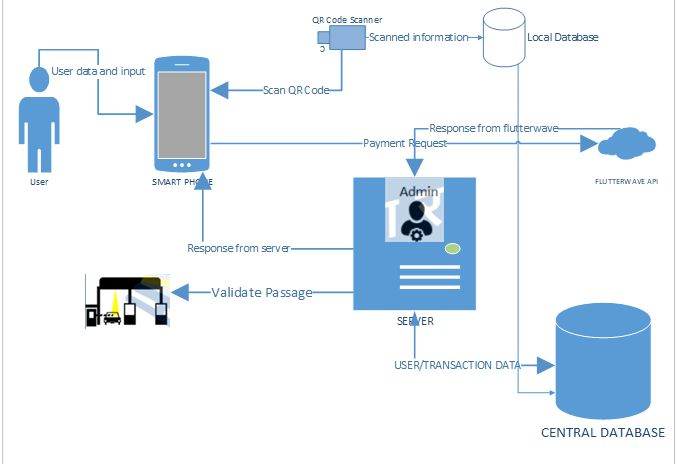
\includegraphics[scale = 0.8]{images/etolssys}
        \caption{System Architecture diagram for E-Tolls System}
    \end{center}
\end{figure}

\subsubsection{Logical Design}
\begin{figure}
    \begin{center}
        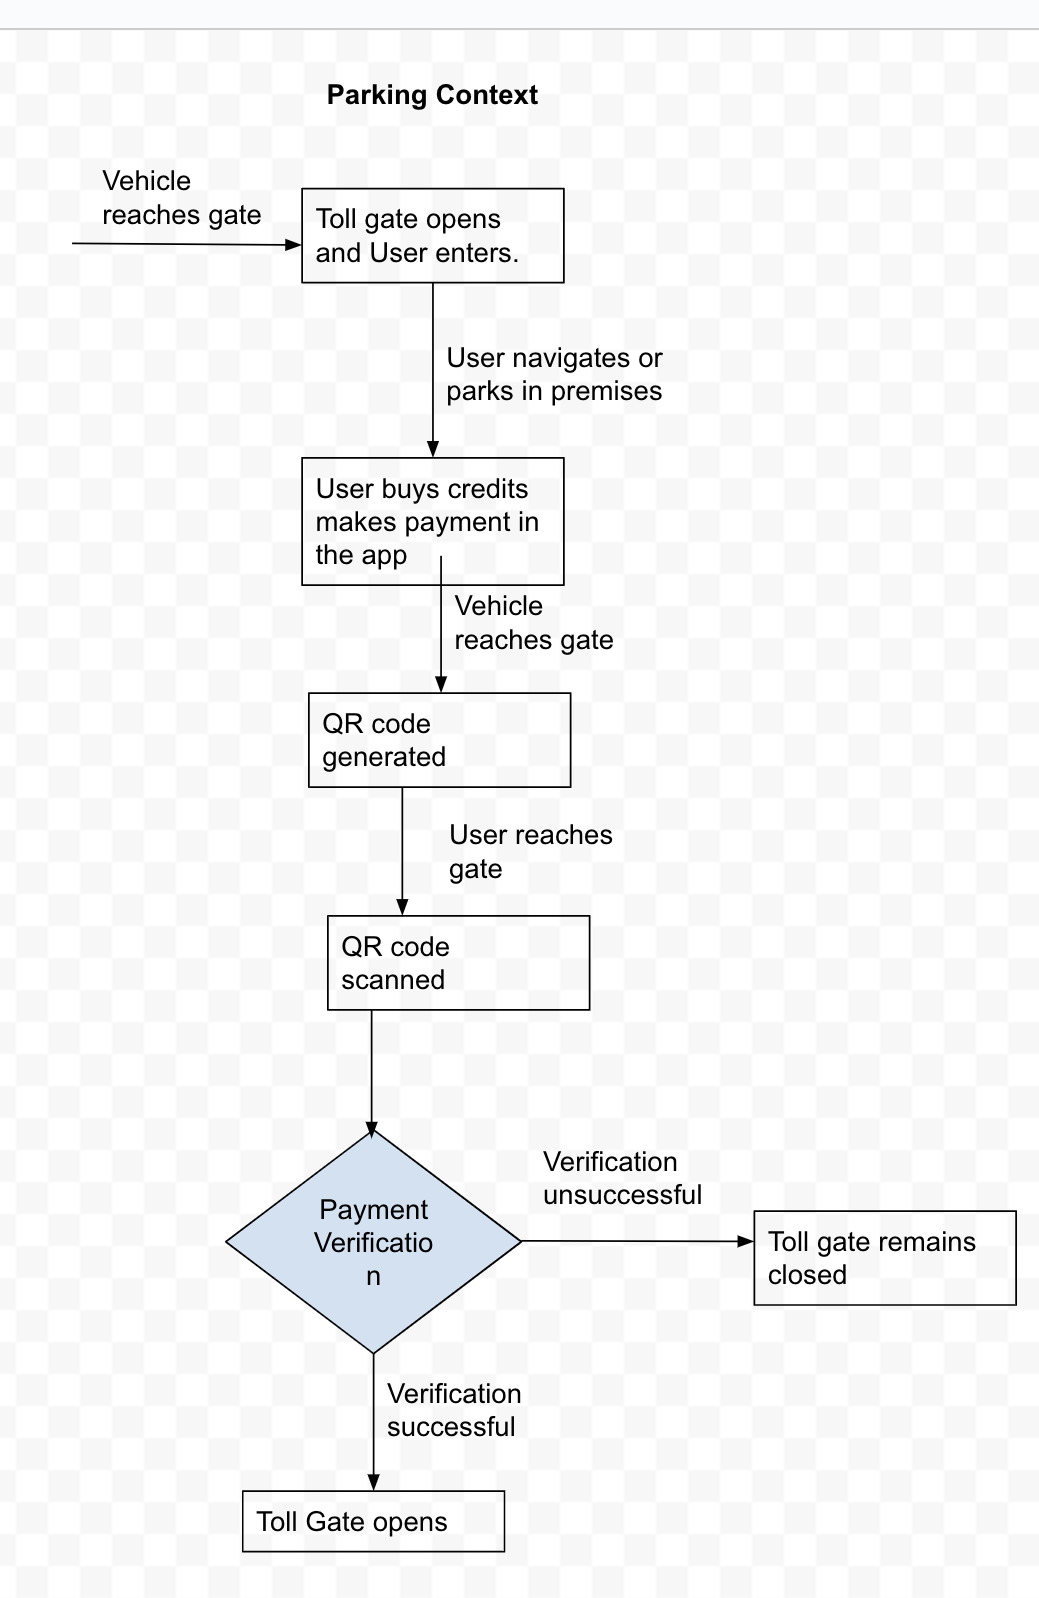
\includegraphics[scale = 0.6]{images/userflowdiagram}
        \caption{System Architecture diagram for E-Tolls System}
    \end{center}
\end{figure}

